\documentclass[letterpaper,10pt]{article}
\usepackage{hyperref}
\usepackage[margin=1in]{geometry}
\usepackage{amsmath}
\usepackage{amssymb}
\usepackage{amsthm}
\usepackage{mdframed}
\usepackage{enumitem}
\usepackage{tikz}
\usepackage{graphicx}
\usepackage{wrapfig}
\usepackage{subcaption}

%%%%% TIKZ packages
\usetikzlibrary{external}\tikzexternalize
\author{Connor Duncan}
\title{Math 222B Notes}
\date{\today}

%%%%% MATH COMMANDS
\newcommand{\wkp}{W^{k,p}}
\newcommand{\lsim}{\lesssim}
\DeclareMathOperator{\spt}{spt}
\DeclareMathOperator{\rg}{range}
\DeclareMathOperator{\img}{img}
\DeclareMathOperator{\dist}{dist}
\DeclareMathOperator{\tr}{tr}
\DeclareMathOperator{\ext}{ext}
\DeclareMathOperator{\id}{id}
%%%%% TODO:
% Citations

%%%%% DEFINITION
\theoremstyle{definition}
\newtheorem{dfn}{Definition}
\newtheorem*{ntt}{Notation}

\theoremstyle{remark}
\newtheorem*{rmk}{Remark}
\newtheorem*{eg}{Example}

%%%%% THEOREM
\theoremstyle{plain}
\newtheorem{thm}{Theorem}[section]
\newtheorem{prop}[thm]{Prop}
\newtheorem{lem}[thm]{Lemma}

%%%%% PROOF ENVIRONMENT
%%% Proofs from lecture/text
\newenvironment{proofm}{
    \vspace{5pt}
    \begin{mdframed}[
        bottomline=false,topline=false,rightline=false, linecolor=red,linewidth=2pt, skipabove=0
    ]
    \noindent\textit{Proof.}
}{
    \hspace{\fill}\qedsymbol\end{mdframed}
}
\renewenvironment{proof}{
    \vspace{5pt}
    \begin{mdframed}[bottomline=false,topline=false,rightline=false, skipabove=0]
    \noindent\textit{Proof.}}
{
    \hspace{\fill}\qedsymbol
    \end{mdframed}
}

%%%%% DOCUMENT
\begin{document}
\maketitle
\tableofcontents

\section{Sobolev Spaces}
The reference for this section is Evans Chapter 5., and Sung-Jin Oh's 222A lecture
notes, section 11.

\subsection{Introduction to Sobolev Spaces} %TODO: ask prof Oh about this distinction w/the 1/p's
We begin with an introduction to the basics of Sobolev Spaces.
\begin{dfn}
    Let $U$ be an open subset of $\mathbb R^d$, and $u\in\mathcal D'(U)$.
    The $k^{\text{th}}$ order $L^p$-based Sobolev Norm of $u$ is defined as:
    $$
    ||u||_{W^{k,p}{U}}=\left[\sum_{\alpha:|\alpha|<k}^{}||D^\alpha u||_{L^p(U)}^p\right]^{1/p}
    $$
    Here, $D^\alpha$ is the weak derivative, and $D^\alpha u\in L^p(U)$.\footnote{This is equivalent to the other definition given in lecture:
        $||u||_{\wkp(U)}=\sum_{\alpha:|\alpha|<k}^{}||D^\alpha u||_{L^p(U)}$.
        % TODO prove equivalence?
    }
\end{dfn}

\begin{rmk}
    The sum over $||D^\alpha u||_{L^p}$ is motivated by its appearance in 
    energy-method solutions to PDE's found in 222A.
\end{rmk}

\begin{dfn}
    The $L^p$-Sobolev space of order $k$ on $U$ is defined as
    $$
    W^{k,p}(U)=\{u\in\mathcal D'(U):||u||_{W^{k,p}(U)}<\infty\}
    $$
    Similarly, we call the subspace of $W^{k,p}(U)$ which vanish to appropriate 
    order on the boundary
    $$
    W_0^{k,p}(U)=\overline{C_c^\infty(U)}^{||\cdot||_{W^{k,p}(U)}}\subset W^{k,p}(U)
    $$
\end{dfn}
When $p=2$, we have many extra analytical tools, since the Fourier transform
is an $L^2$ isometry. This justifies special notation for this case.
\begin{ntt}
    We denote by $H^k(U)=W^{k,2}(U)$, and $H_0^k(U)=W_0^{k,2}(U)$.
\end{ntt}
We also have a special notation for inequalities that hold up to a multiplicative
constant.
\begin{ntt}
    If, for some $c>0$, $A\leq cB$, then $A\lsim B$.
    If $A\lsim B$ and $B\lsim A$, then $A\simeq B$.
\end{ntt}
\begin{prop}\label{prop:wkpbasics}
    Some basic facts about $W^{k,p}(U)$ and $H^k(U)$.
    \begin{enumerate}[label=\roman*.]
        \item For all $k\in\mathbb Z_{\geq 0}$ and $1\leq p\leq\infty$,
            $(\wkp(U),||\cdot||_{W^{k,p}(U)})$ and $(\wkp_0(U),||\cdot||_{\wkp})$
            are Banach spaces.

        \item For all $k\in\mathbb Z_{\geq 0}$, and denoting 
            $\langle u,v\rangle_{H^k(U)}=
            \sum_{\alpha:|\alpha|\leq k}^{}\langle D^\alpha u,D^\alpha v\rangle_{L^2(U)}$,
            both $(H^k(U),\langle\cdot,\cdot\rangle_{H^k(U)})$ and
            $(H^k_0(U),\langle\cdot,\cdot\rangle_{H^k(U)})$ are Hilbert Spaces.

        \item (Fourier Analytic Characterization of $H^k$). If $u\in H^k(U)$,
            then $||u||_{H^k}\simeq ||\hat u||_{L^2}+|||\xi|^k\hat u||_{L^2}
            \simeq ||(1+|\xi|^2)^{k/2}\hat u||_{L^2}$.
    \end{enumerate}
\end{prop}
\begin{proofm} %TODO: i,ii are partially due to evans.
    For ($i$), we first check that $||\cdot||_{\wkp}$ is a norm.
    The triangle inequality may be verified by the elementary calculation, where $u,v\in\wkp$:
    \begin{align*}
        ||u+v||_{\wkp}=\left[\sum_{\alpha:|\alpha|\leq k}^{}||D^\alpha(u+v)||_{L^p}^p\right]^{1/p}\\
        \leq\left[\sum_{\alpha:|\alpha|\leq k}^{}(||D^\alpha u||_{L^p}+||D^\alpha v||_{L^p})^p\right]^{1/p}\\
        \leq\left[\sum_{\alpha:|\alpha|\leq k}^{}||D^\alpha u||_{L^p}^p\right]^{1/p}
        +\left[\sum_{\alpha:|\alpha|\leq k}^{}||D^\alpha v||_{L^p}^p\right]^{1/p}
        \\
        =||u||_{\wkp}+||v||_{\wkp}
    \end{align*}
    The first inequality follows from the fact that $||\cdot||_{L^p}$ is a norm.
    It is obvious that $||\lambda u||_{\wkp}=|\lambda|||u||_{\wkp}$.

    It remains to check that $\wkp$ is complete. Let $\{f_n\}_1^\infty$ be a Cauchy
    sequence in $\wkp$.
    By definition, every $D^\alpha f_i\in L^p$, and since $L^p$ is complete 
    every $D^\alpha f_i$ converges to a function $f_\alpha\in L^p$.
    So, the claim is that when $\alpha=(0,\ldots,0)$, we have convergence in $L^p$:
    $f_m\rightarrow f_{(0,\ldots,0)}:=f\in\wkp$.
    To see that $f\in\wkp$, fix a test function $\phi\in C^\infty_0$, and integrate
    \begin{align*}
        \int_{}^{}fD^\alpha\phi dx=\lim_{n\rightarrow\infty}\int_{}^{}f_nD^\alpha\phi dx\\
        =\lim_{n\rightarrow\infty}(-1)^{|\alpha|}\int_{}^{}(D^\alpha f_n)\phi dx
        \\
        =(-1)^{|\alpha|}\int_{}^{}f_\alpha \phi dx
    \end{align*}
    This shows that every Cauchy sequence of functions and all derivatives of index 
    $|\alpha|<k$ converge in $L^p$, which proves convergence in $W^{k,p}$.
    For $\wkp_0$, we need only check that $f_\alpha$ is compactly supported for all
    $\alpha$. This is easily accomplished by replacing $\phi$ with $\varphi\in C^\infty$,
    and repeating the calculaton.

    For ($ii$), we first check that $\langle\cdot,\cdot\rangle_{H^k}$ is an inner product.
    Letting $a,b\in\mathbb C$, and $f,g,h\in H^k$, we have
    \begin{align*}
        \langle af+bg,h\rangle_{H^k}
        =\sum_{\alpha:|\alpha|\leq k}^{}\langle D^\alpha(af+bg),D^\alpha h\rangle_{L^2}\\
        =\sum_{\alpha:|\alpha|\leq k}^{}a\langle D^\alpha f,D^\alpha h\rangle_{L^2}+b\langle D^\alpha g,D^\alpha h\rangle_{L^2}\\
        =a\langle f,h\rangle_{H^k}+b\langle g,h\rangle_{H^k}
    \end{align*}
    That $\langle y,x\rangle_{H^k}=\overline{\langle x,y\rangle_{H^k}}$ follows 
    from the same fact for the $L^2$ inner product, as does positivity.
    Completeness follows from ($i$), which shows that $(H^k,\langle\cdot,\cdot\rangle_{H^k})$ 
    is a Hilbert space.

    For $(iii)$, we have to use some properties of the Fourier transform proved in
    222A. Let $u\in H^k$. %TODO: shouldn't some of these be square?
    Since $u\in L^2$, we may write that $\widehat{(D^\alpha u)}=
    ((i\xi)^\alpha\hat u)$. 
    Clearly, we have that $||u||_{H^k}\geq C||\hat u||_{L^2}+|||\xi|^k\hat u||_{L^2}$,
    since the latter quantity contains only some of the terms present in the $H^k$ norm.
    That $||\hat u||_{L^2}+|||\xi|^k\hat u||_{L^2}\geq C||(1+|\xi|^2)^{k/2}\hat u||_{L^2}$
    follows from the Cauchy-Schwarz inequality and because $|\xi|>0$, we have 
    $(1+|\xi|^2)^{k/2}\leq C(1+|\xi|^2)^{k/2}$.
    From this, the chain of inequalities (choosing appropriate $C$ so that all constant-dependent
    inequalities still hold) reads as
    $$
    ||u||_{H^k}\geq C\left(||\hat u||_{L^2}^2+|||\xi|^k\hat u||_{L^2}^2\right)^{1/2}
    \geq C||(1+|\xi|^k)\hat u||_{L^2}\geq ||(1+|\xi|^2)^{k/2}\hat u||_{L^2}
    $$
    All that remains is to show that $||(1+|\xi|^2)^{k/2}\hat u||_{L^2}\geq C||u||_{H^k}$.
    To see this, note that $(1+|\xi|^2)^{k/2}=\sum_{j=0}^{k/2}c_j|\xi|^{2j}$, pick the 
    smallest $C=c_j$, and doing this once more for the sum that appears,
    $$
    ||(1+|\xi|^2)^{k/2}\hat u||_{L^2}^2\geq C||\sum_{j=0}^{k}|\xi|^j\hat u||_{L^2}^2
    \geq C'\sum_{\alpha:|\alpha|\leq k}^{}||D^\alpha u||_{L^2}^2
    $$
    Taking a square root completes the proof.
\end{proofm}
Naturally, for a vector space like $\wkp(U)$, we ask what the dual of this 
space is. By an appropriate definition, we can characterize the dual 
as being a Sobolev space of negative order.
\begin{dfn}
    For $k\in\mathbb Z_{\geq 0}$, $1<p<\infty$, and $U$ and open subset 
    of $\mathbb R^d$, we define
    $$
    ||u||_{W^{-k,p}(U)}=\inf\left\{\sum_{\alpha:|\alpha|<k}^{}||g_\alpha||_{L^p(U)}:u=\sum_{\alpha:|\alpha|<k}^{}D^\alpha g_\alpha\right\}
    $$
    and 
    $$
    W^{-k,p}(U)=\left\{u\in\mathcal D'(U):u=\sum_{\alpha:|\alpha|<k}^{}D^\alpha g_\alpha, g_\alpha\in L^p(U)\right\}
    $$
\end{dfn}

\begin{rmk}
    If $g\in L^p(U)$, then $D_{x^i}g\in W^{-1,p}(U)$.
    If $g\in\wkp(U)$, then $D_{x^i}g\in W^{k-1,p}(U)$.
    In essence, we can characterize $W^{-k,p}$ as the space of $L^p$ functions
    weakly differentiated up to $k$ times.
\end{rmk}
With this in mind, we are able to prove the following proposition.
\begin{prop}
    For $k\in\mathbb Z_{\geq 0}$, $1\leq p\leq\infty$, and $p'$ such that 
    $\frac{1}{p}+\frac{1}{p'}=1$,
    $$
    (\wkp_0(U))^*\simeq W^{-k,p'}(U)
    $$  
\end{prop}
\begin{proof} %TODO: could probably be cleaned up.
    We show first that $(\wkp_0)^*\supseteq W^{-k,p'}(U)$. 
    Let $v\in W^{-k,p'}(U)$, and $u\in\wkp_0(U)$.
    By definition, we may write $v=\sum_{\alpha:|\alpha|<k}^{}D^\alpha g_\alpha$.
    Testing $v$ against $u$, we find that 
    \begin{align*}
        \langle v,u\rangle=\int_{U}^{}vudx
        =\sum_{\alpha:|\alpha|<k}^{}\int_{U}^{}D^\alpha g_\alpha u dx
        =\sum_{\alpha:|\alpha|<k}^{}\int_{U}^{}(-1)^\alpha g_\alpha D^\alpha udx
        \\
        \leq\sum_{\alpha:|\alpha|<k}^{}||g_\alpha||_{L^{p'}}||D^\alpha u||_{L^p}
        \\
        \leq c||v||_{W^{-k,p'}}||u||_{\wkp} 
    \end{align*}
    Here, the third equality follows by integrating by parts, using the fact that 
    $\spt(u)$ is compact in $U$ to disregard boundary terms.
    The first inequality is a direct application of H\"older's inequality (\ref{thm:holderineq}).
    The second is the definition of the Sobolev norm, aggregating the 
    constants from each term into $c$.  
    Thus, we have shown that every $v$ in $W^{-k,p'}(U)$ is a bounded linear functional
    on $\wkp_0$, i.e. an element of the dual space.

    To show that $(\wkp_0)^*\subset W^{-k,p'}$, we apply the Hahn-Banach theorem (\ref{thm:hahnbanach}).
    First, define the bounded linear functional $\ell:\wkp_0\rightarrow\mathbb R$,
    and let $u\in C_0^\infty(U)$, with the end goal that $\ell(u)=\langle v,u\rangle
    =\sum_{\alpha:|\alpha|<k}^{}(-1)^\alpha\langle g_\alpha, D^\alpha u\rangle$.
    To that end, we define (where $K(k)$ is the total number of multi-indices
    up to order $k$):
    $$
    \begin{matrix}
        T:  &   C_0^\infty(U)\rightarrow L^p(U)^{K(k)}\\
        &   u\mapsto (u,D_{x^1}u,\ldots,D_{x^d}u,\ldots D^\alpha u) 
    \end{matrix}
    $$
    We have that $||T(u)||\leq c||u||_{\wkp}$.
    Furthermore, $T$ is injective, and an isomorphism onto its image, i.e.,
    $(C_0^\infty(U),||\cdot||_{\wkp})\sim(T(C_0^\infty(U)), ||\cdot||)$.
    So, we may send $\ell$ to $\tilde\ell:T(C_0^\infty(U))\rightarrow\mathbb R$
    by composing with this isomorphism.
    In particular, $\tilde\ell(Tu)=\ell(u)$ tells us that $\tilde\ell$ is similarly
    bounded.
    Now, by the Hahn-Banach theorem, $\tilde\ell$ extends to the bounded linear
    functional $\tilde{\tilde\ell}:(L^p(U))^{\otimes K}\rightarrow\mathbb R$.
    By definition, $\tilde{\tilde\ell}\in \left((L^p(U))^{\oplus K}\right)^*
    =\{\tilde v=\sum_{\alpha:|\alpha|<k}^{}\tilde g_\alpha:\tilde g_\alpha\in L^{p'}(U)\}$.
    So, for some $\tilde u\in (L^{p}(U))^{\oplus K}$, the pairing with $\tilde v$ is 
    exactly $\langle\tilde v,\tilde u\rangle=\sum_{\alpha:|\alpha|<k}^{}\langle g_\alpha,u_\alpha\rangle$,
    where $\tilde u_\alpha=D^\alpha u$.
    So,
    $$
    \ell(u)=
    \tilde\ell(Tu)=\tilde{\tilde\ell}(Tu)
    =\sum_{\alpha:|\alpha|<k}^{}\langle\tilde g_\alpha, (Tu)\alpha\rangle
    =\sum_{\alpha:|\alpha|<k}^{}\langle\tilde g_\alpha, D^\alpha u\rangle
    $$
    If we choose $g_\alpha=(-1)^{|\alpha|}\tilde g_\alpha$, we have shown
    the remainder of the proof.
\end{proof}

\subsection{Existence and Uniqueness Problems}
The concrete objective of this section is to explore the duality relationship 
between the existence and uniqueness of solutions to linear equations
on Banach spaces. In particular, apriori estimates of the dual
problem prove the existence of solutions to the direct problem, and vice-versa (under
certain conditions).
\begin{prop}\label{prop:dual1}
    Let $X,Y$ be Banach Spaces, and let $P:X\rightarrow Y$ be a bounded linear
    operator. Likewise, let $P^*:Y^*\rightarrow X^*$ be the adjoint of $P$.
    Suppose that there exists $c>0$ such that $||u||_X\leq c||Pu||_Y$ for all $u\in X$.
    Then the following hold:
    \begin{enumerate}[label=\roman*.]
        \item (Uniqueness for $Pu=f$) If $u\in X$, $Pu=0\Rightarrow u=0$.
        \item (Existence for $P^*v=g$) For all $g\in X^*$, there exists 
            $v\in Y^*$ such that $P^*v=g$, and $||v||_{Y^*}\leq c||g||_{X^*}$.
    \end{enumerate}
\end{prop}
\begin{proof}
    The proof of $(i)$ is clear, since $||u||_{X}\leq 0$, $u=0$ since $X$ is normed.

    As for $(ii)$, we again apply the Hahn-Banach theorem. In particular, our objective
    is to find $v\in Y^*$ such that for all $u\in X$:
    $P^*v=g\Leftrightarrow\langle P^*v,u\rangle=\langle g,u\rangle=\langle v, Pu\rangle$.
    To that end, define $\ell:P(X)\rightarrow\mathbb R$, where $\ell(Pu)=\langle g,u\rangle$.
    Since $P$ is injective by $(i)$, $\ell$ is well-defined.
    By definition, if $||Pu||_Y\leq 1$, we have that 
    $$
    |\ell(Pu)|=|\langle g,u\rangle|\leq||g||_{X^*}||u||_X
    \leq c||g||_{X^*}||Pu||_Y
    \leq c||g||_{X^*}
    $$
    So, by the Hahn-Banach theorem, there exists $v\in Y^*$ such that 
    $\langle v,Pu\rangle=l(Pu)=\langle g,u\rangle$ for all $u\in X$, 
    and $||v||_{Y^*}\leq c||g||_{X^*}$.
\end{proof}
\begin{dfn}
    Let $X$ be a normed vector space with member $x$, 
    and let $\hat x:X^*\rightarrow\mathbb C$ denote
    $\hat x(f)=f(x)$. Let $\hat X=\{\hat x:x\in X\}$.
    $X$ is called \textbf{reflexive} if $\hat X=X^{**}$. 
\end{dfn}
If we want existence for the direct problem, we take the easy way, and assume $X$
is reflexive, which yields Proposition \ref{prop:dual2}.
In general, $\hat X\subseteq X^{**}$.
\begin{prop}\label{prop:dual2}
    Let $X,Y$ be Banach Spaces, with $X$ reflexive, 
    and Let $P:X\rightarrow Y$ be a bounded linear operator.
    Likewise, let $P^*:X^*\rightarrow Y^*$ be the adjoint of $P$.
    Suppose that there exists $c>0$ such tht $||v||_{Y^*}\leq c||P^*v||_{X^*}$.
    Then the following hold:
    \begin{enumerate}[label=\roman*.]
        \item (Uniqueness for $P^*v=g$) If $v\in Y^*$, $P^*v=0\Rightarrow v=0$.
        \item (Existence for $Pu=f$) For all $f\in Y$, there exists 
            $u\in X$ such that $Pu=f$, and $||u||_{X}\leq c||f||_{Y}$.
    \end{enumerate}
\end{prop}
\begin{proofm}
    Exercise.
\end{proofm}

\begin{rmk}
    All Sobolev Spaces $\wkp_0$ for $1<p<\infty$ are reflexive. This will be a
    homework problem.
\end{rmk}

\begin{ntt}
    Let $P:X\rightarrow Y$ be a linear operator, and $P^*$ its associated adjoint.
    With $U\subset Y$, and $V\subset X^*$, we define the following sets:
    \begin{align*}
        U^\perp=\{v\in Y^*:\langle v,f\rangle=0\, \forall f\in U\}
        \\
        ^\perp V=\{u\in X:\langle g,u\rangle=0\, \forall g\in V\}
    \end{align*}
\end{ntt}
\begin{rmk}
    $\rg(P)^\perp=\ker(P^*)$, and $\ker(P)=^\perp\rg(P^*)$. 
    As a consequence of this fact, if $\ker P^*=\{0\}$, 
    then $\rg(P)^\perp=\{0\}\Leftrightarrow\overline{\rg(P)}=Y$.

    It's worth noting that in finite dimensions, $\overline{\rg(P)}=\rg P$,
    which provides the simpler duality relation between uniqueness and existence
    of solutions for linear operators.
    In infinite dimensions, this does not always hold, which is what our boundedness
    estimate provides. There is no loss of generality for deriving existence for $P$
    from the qualitative bound
    \begin{equation}\label{eq:qbound}
        ||v||_{Y^*}\leq c||P^*v||_{X^*}
    \end{equation}
\end{rmk}
\begin{ntt}
    We denote by $B_X=\{x\in X:||x||_X<1\}$.
\end{ntt}
\begin{prop}\label{prop:uqexistest}
    Let $X,Y$ be Banach Spaces, and $P:X\rightarrow Y$ a bounded linear operator.
    If $P(X)=Y$, then there exists $c>0$ such that (\ref{eq:qbound}) holds.
\end{prop}
\begin{proof}
    $||P^*v||_{X^*}=\sup_{\overline{B_X}}|\langle P^*v,u\rangle|=\sup_{\overline{B_X}}|\langle v, Pu\rangle|$.
    $T$ is a surjective linear map between Banach spaces, and is therefore open by the 
    Open mapping theorem (\ref{thm:openmap}).
    Thus, $P(B_X)$ is open and contains $0$. Thus, there exists $c>0$ such that 
    $P(B_X)\supseteq cB_Y$, which implies
    $$
    ||P^*v||_{X^*}=\sup_{\overline{B_X}}|\langle P^*v,u\rangle|
    =\sup_{\overline B_X}|\langle v,Pu\rangle|
    \geq
    \sup_{f\in cB_Y}|\langle v,f\rangle|=c||v||_{Y^*}
    $$
    which completes the proof.
\end{proof}

\begin{eg}
    We now examine the solvability of the equation $-u''=f$ in $H_0^1((0,1))$.
    Note that $||u||^2_{H^1}=||u||^2_{L^2}+||u'||^2_{L^2}$, and that 
    $(H_0^1)^*=H^{-1}$.
    Using $X=H_0^1, Y=H^{-1}$, we consider $P=-\partial_x^2$, and claim that 
    if $-u''=f$ for $u\in H_0^1$, then $$||u||_{H^1}\leq c||f||_{H^{-1}}.$$
    The proof is an application of the energy method.
    A simple integration by parts yields that 
    $$
    \int_{}^{}-u''udx=\int_{}^{}fudx=\int_{}^{}(u')^2dx=||u'||^2_{L^2}
    $$
    To obtain the previous inequality from what we have just derived, we use the fact that
    $u$ is zero on the boundary, and so $u(x)=\int_{0}^{x}u'(y)dy$.
    Using the Cauchy-Schwarz inequality,
    $$
    |u(x)|\leq\int_{0}^{1}|u'(y)|dy\leq ||u'||_{L^2}
    $$
    which implies that 
    $$
    \int_{0}^{1}|u|^2dy\leq\sup_{[0,1)}|u|^2\leq||u'||^2_{L^2},
    $$
    in turn implying that 
    $$
    ||u||^2_{H^1}\leq c|\langle f,u\rangle|\leq c||f||_{H^{-1}}+||u||_{H^1}
    $$
    which completes the proof after dividing out a term $||u||_{H^1}$.

    From this, we can deduce from the inequality above, and Proposition \ref{prop:dual1}
    that $-u''=0$ and $u\in H_0^1\Rightarrow u=0$.
    From the inequality and Proposition \ref{prop:dual2}, we should compute $P^*$,
    and obtain existence for the dual problem.
    Explicitly, we ue the fact that $H_0^1$ is reflexive, and compute
    for $u\in H_0^1$, that 
    $$
    \langle v, Pu\rangle=\int_{0}^{1}v(-u'')dx=\int_{0}^{1}v'u'dx=\int_{0}^{1}-v''udx
    =\langle P^*v,u\rangle
    $$
    So, $P^*=-\partial_x^2$ as well, meaning the problem is entirely self-adjoint, and 
    $Y^*=H_0$ 1. This gives that $\forall f\in H^{-1}$, there exists $u\in H_0^1$ such that 
    $Pu=f$, by applying Proposition \ref{prop:dual2}.
\end{eg}
This hints at the Poincar\'e inequality, which we will explore shortly.

\subsection{Approximation (Density) Theorems}

\subsubsection{Convolution and Mollifiers}
\begin{dfn}\label{dfn:mollifier}
    Let $\varphi\in C^\infty_0(U)$, with $\int_{U}^{}\varphi=1$.
    We define the family of functions $\varphi_\varepsilon(x)=\frac{1}{\varepsilon^d}\varphi\left(\frac{x}{\varepsilon}\right)$.
    Note that $\int_{U}^{}\varphi_\varepsilon dx=1$ for every $\varepsilon$.
\end{dfn}
\begin{lem}\label{lem:mollifier}
    Let $\varphi\in C^\infty_0$, with $\int\varphi dx=1$, $u\in L^p(\mathbb R^d$ 
    where $1\leq p\leq\infty$, and $\varphi_\varepsilon$ as in Definition \ref{dfn:mollifier}.
    As $\varepsilon\rightarrow 0$, $||\varphi_\varepsilon\star u-u||_{L^p}\rightarrow 0$.
\end{lem}
Before proving the lemma, we note that translations are continuous in $L^p$.
\begin{lem}\label{lem:transcont}
    $\lim_{|z|\rightarrow 0}||u(x-z)-u(x)||_{L^p}=0$ for $u\in L^p$.
\end{lem}
\begin{proofm}
    Clearly, the conditions of the dominated convergence theorem are satisfied,
    choosing $u_n$ to be a sequence of functions $u_n(x)=u(x-z_n)$, where $z_n\rightarrow 0$.
    It suffices to dominate $u_n$ by $v(x)=|u(x)|\cdot\mathbf 1_{B_1(x)}$, under the assumption
    that $z_n$ is a sequence which is of distance at most $1$ from $x$.
\end{proofm}
\begin{proof}(Lemma \ref{lem:mollifier})
    Consider:
    \begin{align*}
        \varphi_\varepsilon\star u-u=\int_{U}^{}u(x-y)\varphi_\varepsilon(y)dy-u(x)
        \\
        =\int_{U}^{}(u(x-y)-u(x)\varphi_\varepsilon(y)dy
    \end{align*}
    Therefore,
    \begin{align*}
        ||\varphi_\varepsilon\star u-u||_{L^p}
        =\left\|\int_{U}^{}(u(x-y)-u(x)\varphi_\varepsilon(y)dy\right\|_{L^p}
        \\
        \leq\int_{U}^{}||u(\cdot-y)-u(\cdot)||_{L^p}|\varphi_\varepsilon(y)|dy
    \end{align*}
    The inequality above is a direct application of the Minkowski inequality. %TODO: ref
    First, we note that $\spt(\varphi_\varepsilon)\rightarrow\{0\}$ as $\varepsilon\rightarrow 0$.
    Furthermore, by the $L^p$-continuity of translations, the entire integrand 
    converges to zero.
\end{proof}
\begin{dfn}\label{dfn:parunity}
    A \textbf{partition of unity} on an open set $U\subset\mathbb R^d$ is a family of 
    functions $\{\chi_\alpha\}_{\alpha\in A}$ such that the following hold:
    \begin{enumerate}[nosep]
        \item $\sum_{\alpha\in A}^{}\chi_\alpha(x)=1$ for all $x\in U$.
        \item For every $x\in U$, only finitely many $\chi_\alpha$ are nonzero at $x$.
    \end{enumerate}
    If $\{U_\alpha\}_{\alpha\in A}$ is an open cover of $U$, $\{\chi_\alpha\}_{\alpha\in A}$
    is called \textbf{subordinate to} $\{U_\alpha\}_{\alpha\in A}$ if $\spt\chi_\alpha\subseteq U_\alpha$
    for all $\alpha$.
    If $\chi_\alpha\in C^{\infty}_0$, then $\{\chi_\alpha\}_{\alpha\in A}$ is called
    a \textbf{smooth partition of unity}.
\end{dfn}
\begin{lem}
    Let $\{U_\alpha\}_{\alpha\in A}$ be an open covering of $U\subset\mathbb R^d$.
    Then there exists a smooth partition of unity subordinate to $\{U_\alpha\}_{\alpha\in A}$.
\end{lem}
\begin{proof}
    Largely omitted. To see this, start from a continuous subordinate partition of 
    unity, and mollify it until you get a smooth partition.
\end{proof}

\subsubsection{Density Theorems}
In what follows, we prove four density theorems, and an extension theorem.
The goal is to provide tools for representing members $u\in W^{k,p}(U)$
by objects with prescribed smoothness and support properties.

\begin{thm}\label{thm:density1}
    Let $k\in\mathbb Z_{\geq 0}$, $1\leq p<\infty$. Then
    \begin{enumerate}[label=\roman*.]
        \item $C^\infty(\mathbb R^d)$ is dense in $\wkp(\mathbb R^d)$.
        \item $C^\infty_0(\mathbb R^d)$ is dense in $\wkp(\mathbb R^d)$.
    \end{enumerate}
\end{thm}
\begin{proof} %TODO finish
    $(i)$ is a rote application of mollifiers. $(ii)$ will be homework. The
    main step is to approximate $f$ by $f\chi(1/R)$, with $\chi\in C_c^\infty$,
    and $\chi(0)=1$.
\end{proof}

\begin{thm}\label{thm:density2}
    Let $k\in\mathbb Z_{\geq 0}$, $1\leq p<\infty$, and $U$ be an open set
    in $\mathbb R^d$. Then $C^\infty(U)$ is dense in $\wkp(U)$.
\end{thm}
\begin{proof}
    \begin{wrapfigure}{r}{0.3\textwidth}
        \centering
        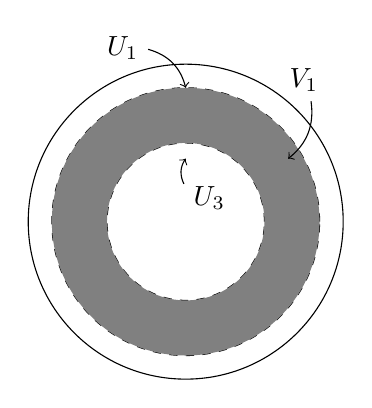
\begin{tikzpicture}
            \node (u1) at (-0.8, 2.2) {$U_1$};
            \node (u3) at (0.3,0.3) {$U_3$};
            \node (v1) at (1.5,1.8) {$V_1$};
            \draw (0,0) circle (2);
            \draw[dashed] (0,0) circle (1.7);
            \draw[dashed] (0,0) circle (1);
            \fill[gray, even odd rule] (0,0) circle (1.7) (0,0) circle (1);
            \draw[->] (u1) to[bend left] (0,1.7);
            \draw[->] (u3) to[bend left] (0,0.8);
            \draw[->] (v1) to[bend left] (1.3,0.8);
        \end{tikzpicture}
        \caption{$U_j$ and $V_j$ in the proof of Theorem \ref{thm:density2}}.
        \label{fig:density2}
    \end{wrapfigure}
    Let $u\in\wkp(U)$, and fix $\epsilon>0$.
    We want to find $v\in C^\infty(U)$ such that $||u-v||_{\wkp(U)}\leq c\epsilon$.
    To that end, consider the family of opens 
    $U_j=\{x\in U:\dist(x,\partial U)<\frac{1}{j}\}$,
    and define $V_j=U_j\setminus\overline{U_{j+2}}$.
    Then, since $U\subseteq\bigcup_{j=1}^\infty V_j$, we may choose $\chi_j$
    to be a partition of unity of $U$ subordinate to $V_j$,
    and write 
    $$
    u=\sum_{j=1}^{\infty}u\chi_j:=\sum_{j=1}^{\infty}u_j
    $$
    Note that because $\spt\chi_j\subseteq V_j$, $\spt u_j\subseteq V_j$,
    Furthermore, $u_j\in C^\infty_0(\mathbb R^d)$, since it is smoothly extended
    by $0$ outside $V_j$.

    Now, we define a mollifier $\varphi \in C_0^\infty(\mathbb R^d)$,
    with the usual $\int_{}^{}\varphi dx=1$, and $\spt\varphi\subseteq B_1(0)$.
    This automatically gives us that $\spt\varphi_{\varepsilon_j}\subseteq B_{\epsilon_j}(0)$,
    for prescribed $\varepsilon_j$.
    We prescribe $\varepsilon_j$ by defining a new $v_j=\varphi_{\varepsilon_j}*u_j$,
    and choosing each $\varepsilon_j$ so that 
    $||u_j-v_j||_{\wkp(U)}\leq 2^{-j}\epsilon$, and 
    $\spt v_j\subseteq\tilde V_j=U_{j-1}\setminus\overline{U_{j+2}}$.
    With these prescribed, we take $v=\sum_{j=1}^{\infty}v_j$.
    First, $v$ is well-defined since $\tilde V_j$ is locally finite.
    Second, we compute
    $$
        ||v-u||_{\wkp(U)}\leq\sum_{j=1}^{\infty}||v_j-u_j||_{\wkp(U)}
        \leq 2^{-j}\epsilon=c\epsilon
    $$
    So, $v$ has the desired convergence and smoothness properties, so we are done.
\end{proof}
One issue with Theorem \ref{thm:density2} is its lack of control over $v$ 
near the boundary of $U$. We attempt to resolve this in the following theorem,
but first, we define some terms.
\begin{ntt}
    $C^\infty(\overline U)=\{u:U\rightarrow\mathbb R:u$ is the restriction
        of a function $\tilde u\in C^\infty(\tilde U),\tilde U\supseteq\overline U\}$.
\end{ntt}
\begin{dfn}
    We say that $\partial U$ is of class $C^k$ if it is locally the graph of a 
    $C^k$ function.
\end{dfn}
    \begin{figure}
        \centering
        \begin{subfigure}{0.4\textwidth}
        \centering
        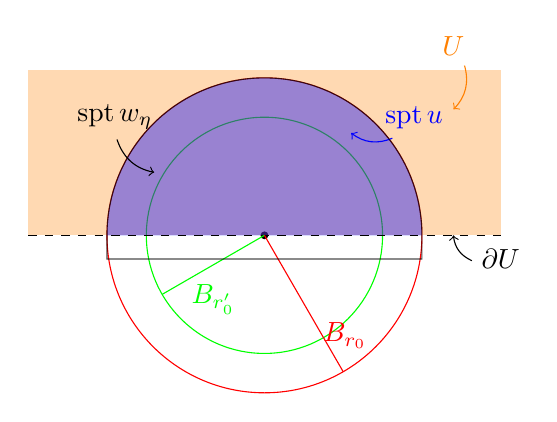
\begin{tikzpicture}
           \draw[red] (0,0) circle (2); 
           \draw[green] (0,0) circle (1.5);
           \fill (0,0) circle (0.05);
           \fill[color=orange,opacity=0.3] (-3,0) -- (3,0) to[color=orange] (3,2.1) to[color=orange] (-3,2.1);
           \fill[color=blue, opacity=0.4] (2,0) arc (180:360:-2) --cycle;
           \draw[dashed] (-3,0) --(3,0);
           \draw[color=green] (0,0) -- ({1.5*cos(210)}, {1.5*sin(210)}) node[midway, label=below:$B_{r'_0}$]{};
           \draw[color=red] (0,0) -- ({2*cos(300)}, {2*sin(300)}) node[midway, label=below right:$B_{r_0}$]{};
           \node[orange] (u) at (2.4,2.4) {$U$};
           \draw[orange,->] (u) to[bend left] (2.4,1.6);
           \node[blue] (sptu) at (1.9,1.5) {$\spt u$};
           \draw[blue,->] (sptu) to[bend left] (1.1, 1.3);

           \draw[opacity=0.7] (2,-0.3) --(2,0) arc (180:360:-2) -- (-2,-0.3) --cycle;
           \node (weta) at (-1.9,1.5) {$\spt w_\eta$};
           \draw[->] (weta) to[bend right] (-1.4,0.8);
           \node (du) at (3,-0.3) {$\partial U$};
           \draw[->] (du) to[bend left] (2.4,0);
        \end{tikzpicture}
        \caption{Illustration of Step 2.}
        \label{fig:density3step2}
        \end{subfigure}
        \hfill
        \begin{subfigure}{0.4\textwidth}
            \centering
            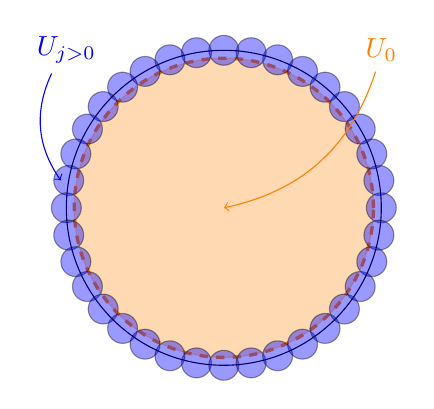
\begin{tikzpicture}
                \draw (0,0) circle (2);
                \draw[dashed,orange,very thick] (0,0) circle (1.9);
                \draw[fill, orange, opacity=0.3] (0,0) circle (1.9);
                \foreach\t in {0,10,...,350}{
                    \draw[fill=blue,opacity=0.4]({2*cos(\t)},{2*sin(\t)}) circle (0.19);
                    %\draw[fill] ({2*cos(\t)},{2*sin(\t)}) circle (0.03);
                }
                \node[color=blue] (uj) at (-2,2) {$U_{j>0}$};
                \draw[color=blue,->] (uj) to[bend right] ({2*cos(170)-0.1},{2*sin(170)});

                \node[color=orange] (u0) at (2,2) {$U_0$};
                \draw[color=orange,->] (u0) to[bend left] (0,0);
            \end{tikzpicture}
            \caption{Open Cover of $U$}
            \label{fig:density3opencover}
        \end{subfigure}
        \caption{Illustration of the proof of Theorem \ref{thm:density3}}
        \label{fig:density3}
    \end{figure}
\begin{thm}\label{thm:density3}
    Let $k\in\mathbb Z_{\geq 0}$, $1\leq p\leq\infty$, and $U$ a bounded
    open subset in $\mathbb R^d$, with $\partial U$ of class $C^1$.\footnote{This can 
    be relaxed to give $U$ a Lipschitz boundary.} %TODO: relax this, and relax boundedness.
    Then $C^\infty(\overline U)$ is dense in $W^{k,p}(U)$.
\end{thm}
\begin{proof}
    The proof proceeds in two steps. The first is to reduce the problem for a
    general $U$ to a region where we may consider $U$ to be the graph of a $C^1$
    function.
    The second is to apply our approximation theorems to these simpler regions,
    before stitching the function back together.
    
    By the definition of $C^1$-regularity, and the fact that $U$ is bounded,
    we may cover $\partial U$ by a finite family of 
    open balls $\{B_{r_j}(x_j)\}_{j=1}^J$, in each of which $U$  may by
    represented as the region above a $C^1$ graph.
    Calling $U_j=B_{r_j}(x_j)$, we choose an open set $U_0$ such that 
    $U\supseteq U_0\supseteq U\setminus\bigcup_{j=1}^J U_j$.
    Then $\{U_j\}_{j=0}^J$ is an open cover of $U$ (which is illustrated in Figure \ref{fig:density3opencover}), so we may take $\{\chi_j\}_{j=0}^J$
    to be a partition of unity subordinate to $U_j$, and--as in the proof of 
    Theorem \ref{thm:density2}--write:
    $$
    u=\sum_{j=0}^{J}u\chi_j:=u_0+\sum_{j=1}^{J}u_j
    $$
    $u_0$ already has compact support, so we are free to apply the previous results.
    For $u_{j>0}$, we need to give a more explicit description of the boundary.

    For this portion, we fix $u=u_j$, and make a change of coordinates so 
    that we are centered at the origin, with $r_0$ and $r_0'$ defined appropriately 
    as in Figure \ref{fig:density3step2}.
    We note that $\partial U=\{x^d=\Gamma(x^1,\ldots x^{d-1}\}$ possibly after 
    a change of coordinates, where $\Gamma$ is the $C^k$ graph function.
    Letting $e^d$ represent the unit coordinate vector in the direction of $x^d$, 
    we make an approximation in two parts.
    First, define $w_\eta(x)=u(x+\eta e^d)$. Note that as $\eta\rightarrow 0$, by
    Lemma \ref{lem:transcont}, $||u-w_\eta||_{\wkp(U\cap B_{r_0})}<\frac{1}{2}\epsilon$
    Moreover, $w_\eta$ is defined on the set $B_{r'_0}\cap U-\eta e^d$.
    Second, we choose $v=\varphi_{r'_0}*w_\eta$, where $\varphi$ is a mollifier.
    Then, for $r'_0\ll\eta$, $v$ is well-defined on $B_{r'_0}\cap\{x^d>\Gamma(x^1,\ldots,x^{d-1})\}$,
    and $||v-w_\eta||_{\wkp(U\cap B_{r_0})}<\frac{1}{2}\epsilon$.
    So, an application of the triangle rule gives that 
    $$
        ||u-v||_{\wkp(U)}\leq\frac{1}{2}\epsilon+\frac{1}{2}\epsilon\leq\epsilon
    $$
    And, since $v\in C^\infty(\overline{V\cap\{x^d>\Gamma(x^1,\ldots, x^d)\}})$,
    we are done.
\end{proof}

\subsubsection{Trace and Extension Theorems}
Extension theorems can be roughly thought of as tools allowing us to handle $u\in\wkp(U)$
when $U$ is a bounded domain.
\begin{thm}\label{thm:extend1}
    Let $k\in\mathbb Z_{\geq 0}$, $1\leq p<\infty$, $U$ a bounded domain in 
    $\mathbb R^d$ with $C^k$ boundary, and $V$ be an open set containing 
    $\overline U$.
    Then there exists $E:\wkp(U)\rightarrow\wkp(\mathbb R^d)$ such that the 
    following hold:
    \begin{enumerate}[label=\roman*.]
        \item (Extension property) $Eu_{|U}=u$.
        \item (Linearity and Boundedness) $E$ is linear, and $||Eu||_{\wkp(\mathbb R^d)}\leq c||u||_{\wkp(U)}$.
        \item (Support) $\spt(Eu)\subseteq V$.
    \end{enumerate}
\end{thm}
\begin{proof}
    Observe that by Theorem \ref{thm:density3}, and the fact that $U$ is bounded,
    it suffices to consider $u\in C^\infty(\overline U)$.
    The proof proceeds in two steps. First, we reduce to the half-ball case, and
    second, we prove extension for the half-ball case.

    To reduce our problem to the case of the half-ball, it suffices to 
    construct an open cover $\{U_0,\ldots, U_J\}$ as in the proof of Theorem
    \ref{thm:density3}, with similarly constructed partition of unity 
    $\{\chi_j\}_{j=0}^J$, and $u_j:=u\chi_j$.
    Notably, $u_0\in\wkp(\mathbb R^d)$ since it is smoothly extended by $0$,
    and $u_k\in C^\infty(\overline U)$, and $\spt u_k\subseteq U_k\cap U$.
    After making a change of coordinates to $y^j=x^j$ for $1\leq j<d$, and 
    $y^d=x^d-\Gamma(x^1,\ldots, x^{d-1})$, we see that 
    $U_k\cap U\mapsto\{y\in B_{\tilde r}(0):y^d>0\}:=\tilde U_k$,
    and $x\mapsto y$ is $C^k$, with smooth $U_j$.
    Therefore, applying the chain rule, we find that $u_j(y)=u_j(x(y))$
    satisfies
    $$
    ||u_j(y)||_{\wkp_y(\tilde U_j)}\leq c||u_k(x)||_{\wkp_x(U_j\cap U)}
    $$
    Thus, it suffices to consider the half-ball case.
    
    \begin{wrapfigure}{r}{0.3\textwidth}
        \centering
        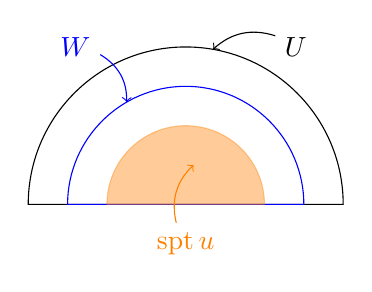
\begin{tikzpicture}
            \node (b0) at (1.4,2) {$U$};
            \node[blue] (bp) at (-1.4,2) {$W$};
            \node[orange] (spt) at (0,-0.5) {$\spt u$};
            \draw (0,0) -- (2,0) arc (0:180:2) -- (0,0);
            \draw[blue] (0,0) -- (1.5,0) arc (0:180:1.5) -- (0,0);
            \draw[fill, orange, opacity=0.4] (1,0) arc (0:180:1) --cycle;
            \draw[->] (b0) to[bend right] ({2*cos(80)},{2*sin(80)});
            \draw[->,blue] (bp) to[bend left] ({1.5*cos(120)},{1.5*sin(120)});
            \draw[->,orange] (spt) to[bend left] (0.1,0.5);
        \end{tikzpicture}
        \caption{Illustration of the proof of Theorem \ref{thm:extend1}.}
    \end{wrapfigure}
    The second step is to actually extend $u$ in the case of the half-ball.
    Here, we define $U=B_r^+(0)$, and $W=B_{r/2}^+(0)$, 
    such that $\spt u\subset W$.
    In order to extend $u$, we use the higher order reflection method,
    defining:
    $$
        Eu=\tilde u=\left\{
        \begin{matrix}
            u(x)        &   x^d>0\\
            \sum_{j=0}^{k}\alpha_ju(x^1,\ldots,x^{d-1},-\beta_jx^d) &   x^d<0
        \end{matrix}\right.
    $$
    Our objective here is to match up the normal derivatives of $\tilde u$ with $u$
    up to order $k$, i.e. set $u(x^1,\ldots, x^{d-1}, 0+)=\sum_{j=0}^{k}\alpha_ju(x^1,\ldots, x^{d-1},0-)$,
    and likewise for all derivatives $\partial_{x^d}^ju=(-\beta_j)^j\partial_{x^d}u$.
    This sets up the following matrix equation for our coefficients $\alpha$ and $\beta$.
    $$
    \begin{pmatrix}
        1\\\vdots\\\vdots\\1
    \end{pmatrix}
    =
    \begin{pmatrix}
        1   &   \cdots  &   1\\
        -\beta_1    &   \cdots &    -\beta_1\\
        \vdots & \vdots & \vdots\\
        (-\beta_k)^k&\cdots&(-\beta_k)^k
    \end{pmatrix}
    \begin{pmatrix}
    \alpha_0\\\vdots\\\vdots\\\alpha_k
    \end{pmatrix}
    $$ %TODO prove some of this stuff about the vandermonde matrix.
    This is the Vandermonde matrix, and if all $\beta_j$'s are distinct, the matrix
    is invertible, which implies that the existence of $\alpha_1,\ldots,\alpha_k$
    such that the equation holds.
    The existence of such coefficients defines $\tilde u$ on $B_r(0)$, extending
    $u$ and matching up derivatives to order $C^k$.
    Finally, to ensure extension to all of $\mathbb R^d$, we apply a cutoff function (a l\'a Urysohn's lemma)
    $\chi_V$, such that $\chi_V=1$ on $U$, and $\spt\chi_V\subset V$. %TODO this step still isn't totally clear.
\end{proof}
Now, we move on to discussing trace theorems, which essentially revolve around 
the restriction of functions $u\in W^{1,p}(U)$ to $\partial U$.
This is interesting in part because the measure of $\mu(\partial U)=0$,
so using only $L^p$ theory to deal with differentiability on the boundary
gives little help, since $L^p$ equivalence is almost everywhere.
\begin{dfn}
    Let $u\in C^1(\overline U)$, and let $U$ be a domain with $C^1$ boundary.
    Then the \textbf{trace of }$u$ \textbf{on the boundary of} $U$ is defined $\tr_{\partial U}(u)=u_{|\partial U}$.
\end{dfn}
Our objective is to first extend this definition to all of $W^{1,p}(U)$.
We note that $\tr_{\partial U}$ is clearly linear, and will 
often write $\tr$ when $\partial U$ is clear from context.
Furthermore, whenever the $L^p$ norm is used on a manifold of dimension less
than the ambient space, it is assumed that integration is with respect to the 
volume fold of the manifold.
\begin{thm}[Nonsharp Trace Theorem]\label{thm:nonsharptr}
    Let $U$ be a bounded, open subset of $\mathbb R^d$, with $\partial U$ of class
    $C^1$, and $1<p<\infty$.
    Then for $u\in C^1(\overline U)$,
    $$
        ||\tr_{\partial U}u||_{L^p(\partial U)}\lsim||u||_{W^{1,p}(U)}
    $$
    As a consequence of this inequality, the following facts hold:
    \begin{enumerate}[label=\roman*.]
        \item $\tr_{\partial U}$ is extended uniquely by continuity and density
            of $C^1(\overline U)\subseteq W^{1,p}(U)$ to 
            $
            \tr_{\partial U}:W^{1,p}(U)\rightarrow L^p(\partial U)
            $
        \item $u\in W_0^{1,p}\Leftrightarrow\tr_{\partial U}u=0$.
    \end{enumerate}
\end{thm}
\begin{proof}
    Evans section 5.5. %TODO do it or cite
\end{proof}
Note that this extension is \emph{not} surjective. $\img(\tr)\subsetneq L^p(\partial U)$.

We direct our attention to a sharp version of Theorem \ref{thm:nonsharptr} in
the setting where $p=2$.
This opens up the world of Fourier analysis, and eventually leads to the world
of fractional-order Sobolev Spaces.
We prove a Sharp Trace theorem for the half-space $\mathbb R^d_+=\{x\in\mathbb R^d:x^d>0\}$,
and denote $\partial U=\{(x',0)\in\mathbb R^d\}\simeq\mathbb R^{d-1}$.

\begin{ntt}[Fourier Transform]
    The convention used for the Fourier and Inverse Fourier transforms
    is as follows: $\hat u=\int_{}^{}u(x)e^{-ix\xi}dx$, and $u(x)=\int_{}^{}\hat ue^{i\xi x}\frac{d\xi}{2\pi}$.
\end{ntt}
\begin{thm}[Sharp Trace Theorem]\label{thm:sharptr}
    When $u\in C^1(\overline{\mathbb R^d_+})\cap H^1(\mathbb R^d_+)$, we have:
    $$
        ||\tr u||_{H^{1/2}(\mathbb R^{d-1})}\lsim ||u||_{H^1(\mathbb R^d_+)}
    $$
\end{thm}
\begin{proof}
    Let $u$ be as in the Theorem statement. Using Theorem \ref{thm:extend1},
    we may extend $u$ to $\tilde u\in C^1(\mathbb R^d)$ such that 
    $||\tilde u||_{H^1(\mathbb R^d)}\lsim ||u||_{\mathbb R^d_+}$.
    Then, we may write
    $$
        \tr u=u(x',0)=\tilde u(x',0)=\int_{}^{}[\mathcal F_{x^d}\tilde u](x',\xi^d)\frac{d\xi^d}{2\pi}
    $$
    Furthermore,
    $$
    [\mathcal F_{x'}\tr u](\xi')=\int_{}^{}[\mathcal F\tilde u](\xi',\xi^d)\frac{d\xi^d}{2\pi}
    $$
    Using the Fourier characterization from Proposition \ref{prop:wkpbasics},
    we may write
    \begin{flalign*}
        ||\tr u||_{H^s}
        &\simeq ||(1+|\xi'|^2)^{s/2}[\mathcal F_{x'}\tr u](\xi')||_{L^2_{\xi'}}
        \\
        &=\left\|(1+|\xi'|^2)^{s/2}\int_{}^{}[\mathcal F\tilde u](\xi',\xi^d)\frac{d\xi^d}{2\pi}\right\|_{L^2_{\xi'}}
        \\
        &\simeq
        \left\|\int_{}^{}[\mathcal F\tilde u](\xi',\xi^d)(1+|\xi'|^2)^{s/2}d\xi^d\right\|_{L^2_{\xi'}}
        \\
        & =
        \left\|
            \left\|
                [\mathcal F\tilde u](\xi',\xi^d)(1+|\xi'|^d)^{s/2}
                \frac{(1+|\xi'|^2+|\xi^d|^2)^{1/2}}{(1+|\xi'|^2+|\xi^d|^2)^{1/2}}
            \right\|_{L^1_{\xi^d}}
        \right\|_{L^2_{\xi'}}
        \\
        & \leq\left\|
        \left\|
            \frac{(1+|\xi'|^2)^{s/2}}{(1+|\xi|^2)^{1/2}}
        \right\|_{L^2_{\xi^d}}
        \left\|
            (1+|\xi|^2)^{1/2}[\mathcal F\tilde u]
        \right\|_{L^2_{\xi^d}}
        \right\|
        \\ 
        & =\left\|
            \left(\int
            \frac{(1+|\xi'|^2)^s}{1+|\xi'|^2+|\xi^d|^2}d\xi^d
            \right)^{1/2}
            ||(1+|\xi|^2)^{1/2}[\mathcal F\tilde u]||_{L^2_{\xi^d}}
        \right\|_{L^2_{\xi'}}
        \\
        & \leq
        \left(\sup_{\xi'\in\mathbb R^{d-1},s\in\mathbb R}\left[
            \int_{}^{}\frac{(1+|\xi'|^2)^s}{1+|\xi'|^2+|\xi^d|^2}d\xi^d
        \right]
        \right)
        ||u||_{H^1(\mathbb R^d_+)}
        \\
        &\simeq ||u||_{H^1(\mathbb R^d_+)}
    \end{flalign*}
\end{proof}

\begin{thm}[Extension from the Boundary]\label{thm:extend2}
There exists a bounded linear map 
$\ext_{\partial U}:H^{1/2}(\mathbb R^{d-1})\rightarrow H^1(\mathbb R^d_+)$
such that $\tr_{\partial U}\circ\ext_{\partial U}=\id$.
\end{thm}
\newpage
\appendix
\section{Frequently Cited Theorems and Definitions}
\subsection{Real Analysis}
\begin{thm}[Existence of Smooth Partitions of Unity]\label{thm:parunity}

\end{thm}
\subsection{Functional Analysis}
\begin{dfn}
    Let $X$ be a real vector space. A map $p:X\rightarrow\mathbb R$ is called 
    a \textbf{sublinear functional} if it satisfies the following for all $x,y\in X$:
    \begin{enumerate}
        \item $p(x+y)\leq p(x)+p(y)$,
        \item For all $\lambda\geq 0$, $p(\lambda x)=\lambda p(x)$.
    \end{enumerate}
\end{dfn}
\begin{thm}[Hahn-Banach]\label{thm:hahnbanach} %TODO cite Folland
    Let $X$ be a real vector space, $p$ a sublinear functional on $X$, $M$
    a subspace of $X$, and $f$ a linear functional on $M$ such that $f(x)\leq p(x)$
    for all $x\in M$.
    Then there exists a linear functional $F$ on $X$ such that $F(x)\leq p(x)$
    for all $x\in X$, and $F_{|M}=f$.
\end{thm}
\begin{proof}
    The following proof is due to Folland. %TODO cite
    We first show that for $x\in X\setminus M$, $f$ may be extended to a linear functional
    $g$ on $M+\mathbb Rx$ which satisfies $g(y)\leq p(y)$.
    For $y_1,y_2\in M$, we have 
    $$
    f(y_1)+f(y_2)=f(y_1+y_2)\leq p(y_1+y_2)\leq p(y_1-x)+p(x+y_2)
    $$
    Rearranging gives
    $$
    f(y_1)-p(y_1-x)\leq p(x+y_2)-f(y_2)
    $$
    Since this applies to every $y_1,y_2\in M$, we have
    $$
    \sup_{y\in M}\{f(y)-p(y-x)\}\leq\inf_{y\in M}\{p(x+y)-f(y)\}
    $$
    Let $\alpha$ be any number which satisfies
    $$
    \sup_{y\in M}\{f(y)-p(y-x)\}\leq\alpha\leq\inf_{y\in M}\{p(x+y)-f(y)\}
    $$
    and define $g:M+\mathbb Rx\rightarrow\mathbb R$ by $g(y+\lambda x)=f(y)+\lambda\alpha$.
    $g$ is linear by the linearity of $f$ and multiplication by $\lambda$. Furthermore,
    $g_{|M}=f$, since any input in $M$ has $\lambda=0$, which gives $g(y)\leq p(y)$ for $y\in M$.
    Moreover, if $\lambda>0$, and $y\in M$, we have
    $$
    g(y+\lambda x)
    =
    \lambda\left[f\left(\frac{y}{\lambda}\right)+\alpha\right]
    \leq
    \lambda\left[f\left(\frac{y}{\lambda}\right)+p\left(x+\frac{y}{\lambda}\right)-f\left(\frac{y}{\lambda}\right)\right]
    =
    p(y+\lambda x)
    $$
    If instead, we say $\lambda=-\mu<0$,
    $$
    g(y+\lambda x)
    =
    \mu\left[f\left(\frac{y}{\mu}\right)-\alpha\right]
    \leq
    \mu\left[f\left(\frac{y}{\mu}\right)-p\left(-x+\frac{y}{\mu}\right)-f\left(\frac{y}{\mu}\right)\right]
    =
    p(y+\lambda x)
    $$
    So, we have $g(z)\leq p(z)$ for all $z\in M+\mathbb Rx$.

    Importantly, the above logic doesn't really depend on the fact $x\in X\setminus M$.
    If $F$ is any linear extension of $f$, then $F\leq p$ on it's domain, which shows
    that the domain of a maximal linear functional satisfying $F\leq p$ must be $X$.
    The family $\mathcal F$ of linear extensions $F$ of $f$ satisfying $F\leq p$
    is partially ordered by inclusion when we consider maps from subspaces of $X$ to 
    $\mathbb R$ as subsets of $X\times\mathbb R$.
    Since the union of any increasing family of subspaces of $X$ is also a subspace of 
    $X$, the union of a linearly ordered subfamily of $\mathcal F$ also lies in $\mathcal F$.
    So, we may invoke Zorn's lemma to guarantee the existence of a maximal 
    element $F\in\mathcal F$, which completes the proof.
\end{proof}
\begin{thm}[Open Mapping]\label{thm:openmap}
    Let $X,Y$ be Banach spaces. If $T\in L(X,Y)$ is surjective, then $T$ maps open sets
    to open sets.
\end{thm}
\begin{proof}
    See Folland 5.10. %TODO Cite
\end{proof}

\subsection{$L^p$ Spaces}
% TODO completeness of L^p space
\begin{thm}[H\"older's Inequality]\label{thm:holderineq}

\end{thm}
\begin{thm}[Minkowski Inequality]\label{thm:minkowskiineq}

\end{thm}

\section{References}
% TODO: this
\end{document}
